\section{Results and Discussion}

\label{sec:results}

Next we describe the results and test the hypotheses before discussing their implications.\footnote{All results are available at \url{http://www.cin.ufpe.br/~mmr3/icse2013/}} We proceed separately with the two tasks (new requirement and unused variable), reporting results from both rounds.

\subsection{New-requirement tasks}

We plot the times for both new-requirement tasks (1 and~2) with in Figure~\ref{fig:beanplots-nr}. Here we use beanplot batches, where each batch shows individual observations as small horizontal lines---the longest represents the average of that batch---and the density trace forms the batch shape. In the initial experiment (see Round 1 legend in the figure), the slowest time when using emergent interfaces is still faster than the fastest time without. On average, participants accomplished the task \textit{3 times} faster with emergent interfaces. The key results were confirmed in the replication (emergent interfaces is, on average, 3.1 times faster), despite the different student levels. According to an ANOVA test, we obtain statistically significant evidence that emergent interfaces reduce effort in both new-requirement tasks.

\begin{figure}[htp]
\centering
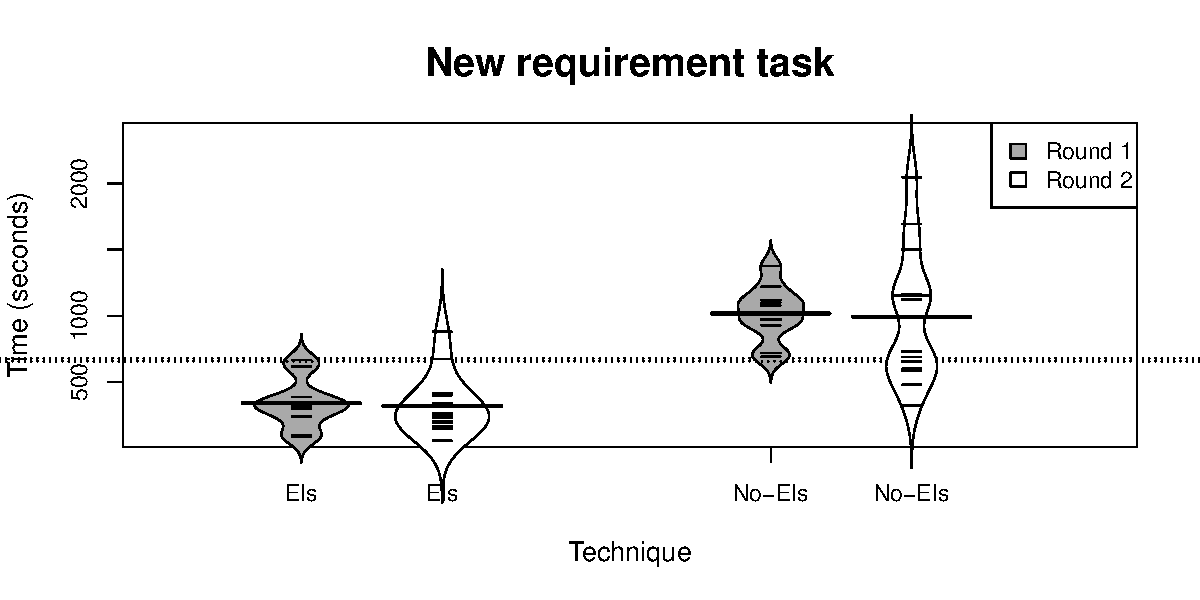
\includegraphics[width=0.5\textwidth]{images/Beanplots-NR.pdf}
\caption{Time results for the new-requirement task in both rounds.}
\label{fig:beanplots-nr}
\end{figure}

In Figure~\ref{fig:barplot-ne}, we plot the NE results for both new-requirement tasks. In Round~1, only one participant committed more errors when using emergent interfaces than without, and all of them committed errors when not using emergent interfaces (they thought they had finished the task but had not, because they potentially missed a dependency). The replication roughly confirms the results: $8$ ($57\%$) participants committed errors when not using emergent interfaces, but only $4$ ($28\%$) participants committed errors with emergent interfaces. Here we do not perform an ANOVA test on number of errors because we have many zero samples, being hard to observe a tendency and draw significant conclusions.

\begin{figure}[htp]
\centering
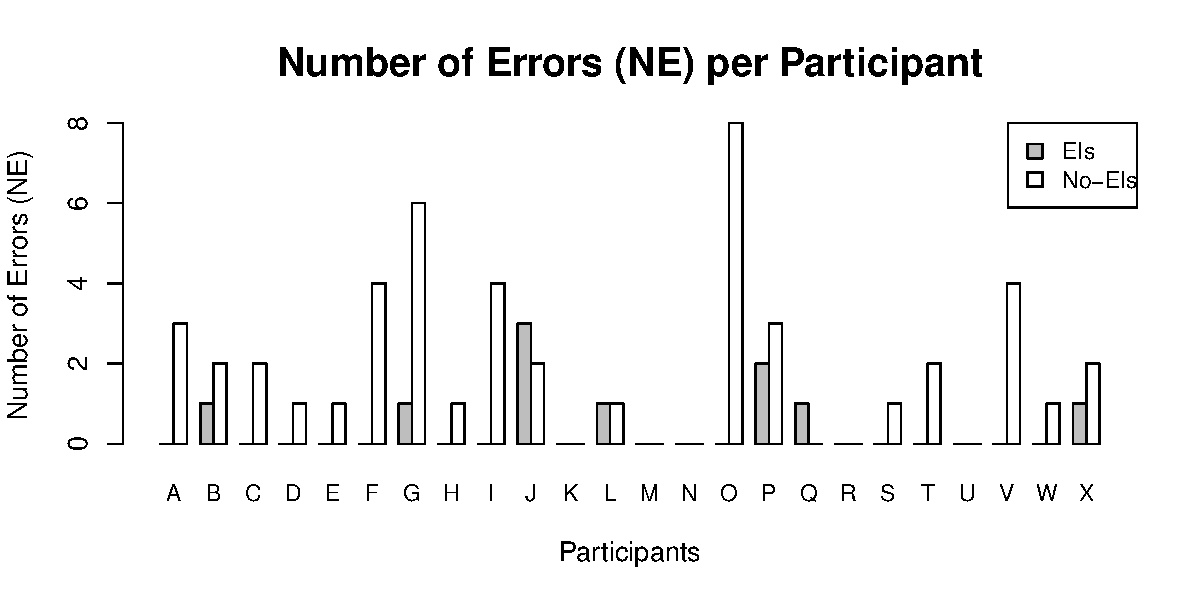
\includegraphics[width=0.5\textwidth]{images/Barplot-NE.pdf}
\caption{Number of Errors for the new-requirement task in both rounds. A-J: Round~1; K-X: Round~2.}
\label{fig:barplot-ne}
\end{figure}

\subsection{Unused-variable tasks}

Differently from the new-requirement task, here we do not have a test case, so we do not force participants to finish the task correctly. Thus, all participants finished the unused-variable task, but some of them committed errors when writing the feature expressions (so, NE $\neq 0$), which means we could have data of participants that, for example, did not try hard enough. In this manner, we assume that, to accomplish the task correctly, participants would need more time and a test case. So, to compensate for the potential lack of effort on performing this task, we test for statistical significance not only the original data, but also data obtained by adding a time penalty (the standard deviation of all participants times) to the participants that perform the task wrongly, adapting the time data.

%to be to able to run the ANOVA test. To do so, we use the standard deviation of all participants times in this task. \chk{REF}

%\chk{seems unsound to me. lets talk about this! if that's standard procedure explain so and give a reference! otherwise we mix our two dependent variables...}

As the unused-variable task consists of fixing two unused variables, we consider it formed by two subtasks. The collected time data corresponds to a participant accomplishing both subtasks. So, we assume that participants spend the same time to accomplish both subtasks and add the time penalty as follows: if NE $= 2$, we add the standard deviation; if NE $= 1$, we add the standard deviation divided by two; if NE $= 0$, we add no penalty.

We plot the adjusted times for both unused-variable tasks (Tasks 3 and~4) in Figure~\ref{fig:beanplots-uv}. Differently from the new-requirement task, here the use of emergent interfaces adds little: the difference between the treatments is smaller. In fact, we obtain statistically significant evidence that emergent interfaces reduce effort only in the second round (this result occurs in both original and adjusted data). Regarding the adjusted time, the participants were {1.6 times} faster, on average.

%In Round~1, participants accomplished the task on average \textit{1.5 times} faster when using emergent interfaces. We confirmed the results in the replication, where participants were \textit{1.6 times} faster. Differently from the \textit{new-requirement} task, here the use of emergent interfaces adds little. We confirm this when running the ANOVA test: the difference between the treatments is not statistically significant on \textit{Round~1}. It is, however, in the replication (\textit{Round~2}).

When considering the product lines peculiarities, the \textit{MobileMedia} methods are simpler when compared to the \textit{Best Lap} ones. The time spent to accomplish the unused-variable task for the \textit{MobileMedia} variables is, on average, fairly similar when using and not using emergent interfaces. However, the difference is much greater for the \textit{Best Lap} variables: participants using emergent interfaces are \textit{2} and \textit{2.2 times} faster in the first and second rounds. Again, notice that the results are similar on both rounds.

%Notice that the difference between VSoC and emergent interfaces is not big when compared to the results of the \textit{new-requirement} maintenance task. On average, when using VSoC, participants are \textit{1.5 times} slower. Three participants ($30\%$) accomplished the maintenance task faster when using VSoC. When considering \textit{Round~2}, the difference is slightly higher: on average, when using VSoC, participants are \textit{1.68 times} slower. Four ($28\%$) participants that were faster when using VSoC.

\begin{figure}[htp]
\centering
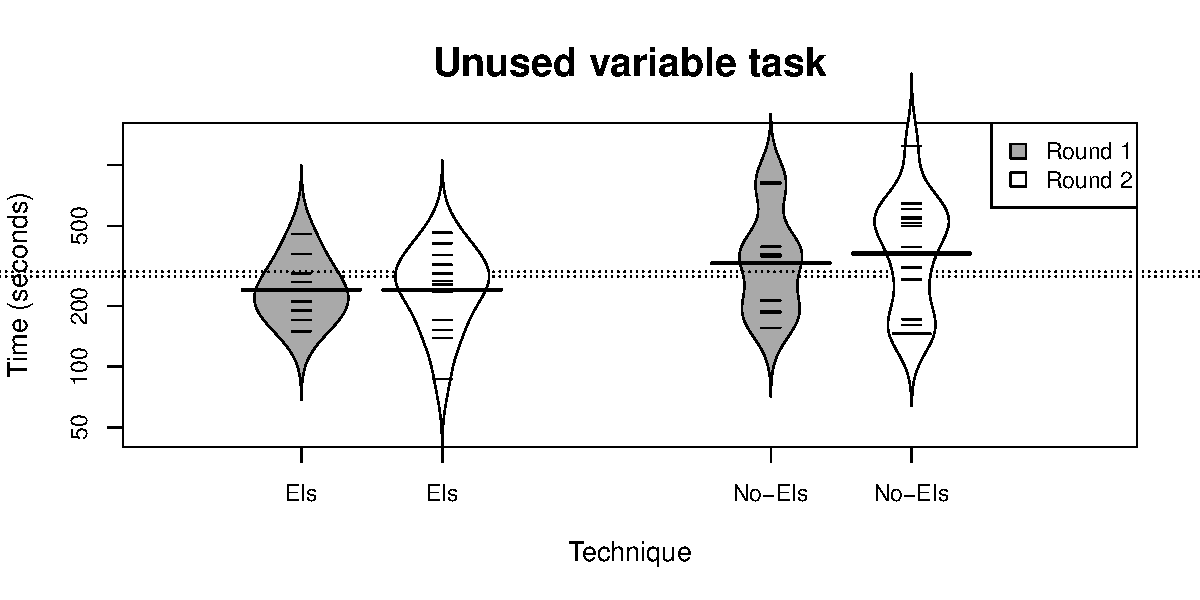
\includegraphics[width=0.5\textwidth]{images/Beanplots-UV.pdf}
\caption{Time results for the unused-variable task in both rounds.}
\label{fig:beanplots-uv}
\end{figure}

%Despite the differences (\textit{1.5} and \textit{1.68}), the ANOVA test points that the first one is not statistically significative (\textit{p-value} $= 0.13$), which leads us to not reject the null hypothesis for \textit{Round~1}. However, we do reject when considering \textit{Round~2}, since the \textit{p-value} for the technique factor is less than $0.05$. In particular, we have \textit{p-value} $= 0.016$.

%According to the Boxplot depicted in Figure~\ref{}, we have an outlier when using VSoC. To verify if this outlier changes our ANOVA test result, we replaced such a value by the VSoC time mean ($\mu = 443$ seconds) and did not add any penalty. Again, we reject the null hypothesis since \textit{p-value} $= 0.024$.

We plot the NE metric in Figure~\ref{fig:barplots-ne2}. The left-hand side represents Round~1; the right-hand side, Round~2. The errors consist of wrongly submitted \texttt{\#ifdef} statements. In general, it turns out that participants commit less errors when using emergent interfaces. The \textit{MobileMedia} methods are simpler, which might explain why participants commit less errors when performing the task in such product line.

\begin{figure}[htp]
\centering
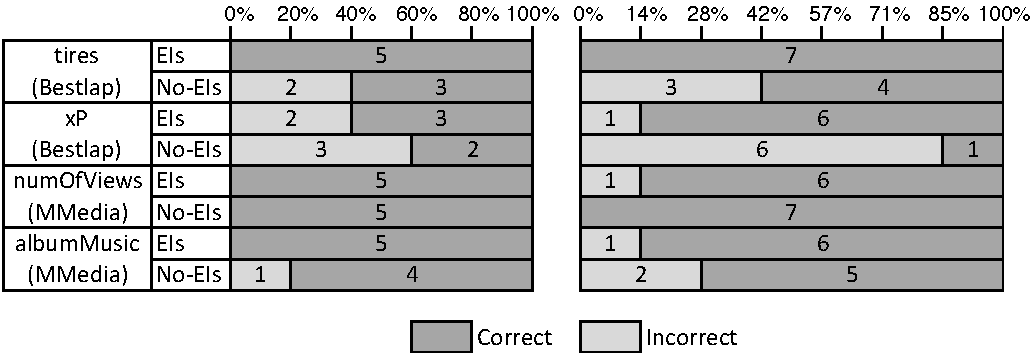
\includegraphics[width=0.5\textwidth]{images/Barplot-NE2.pdf}
\caption{Number of Errors for the unused-variable task in both rounds.}
\label{fig:barplots-ne2}
\end{figure}

To identify other tendencies, we also performed a meta-analysis, jointly analyzing both rounds by  by combining their results. The differences are statistically significant for both tasks.

\subsection{Interpretation}

Regarding Question~1 (\textit{Do emergent interfaces reduce effort during maintenance tasks involving feature code dependencies in preprocessor-based systems?}), we found that emergent interfaces reduce the time spent to accomplish the new-requirement tasks: the difference is large with a three-fold improvement and statistically significant. Despite different student levels (graduate \textit{versus} undergraduate), we confirm our results in both rounds.

Emergent interfaces make feature dependencies explicit and help our participants to concentrate on the task, instead of navigating throughout the code to find and reason about dependencies. Without emergent interfaces, developers need to check for dependencies in every feature. We can see a qualitative difference between new-requirement tasks that require \textit{interprocedural} analysis across several methods and unused-variable tasks that require to analyze code local to a single method. We argue that the effect is not particularly related to the new-requirement task in particular, but rather to tasks containing \textit{interprocedural} dependencies, since they are much more difficult to follow without tool support; finding and reasoning about these dependencies is not straightforward, since they are in different methods and even classes. In contrast, emergent interfaces contribute comparably little over existing search tools when applied in the local context of a function, especially small ones. In fact, we obtain statistically significant evidence in favor of emergent interfaces in only one round. Still on \textit{intraprocedural} context, our results suggest that, depending on the method complexity and size, emergent interfaces adds little. When fixing the unused variables, developers spend fairly the same time (with and without emergent interfaces) on average for \textit{MobileMedia} variables. However, they are, on average, 2 times faster with emergent interfaces for the \textit{Best Lap} variables, which are placed at longer methods.

Emergent interfaces can also help when reasoning about an external feature model Emergo can easily incorporate that information. Also in situations in which Emergo reports an empty interface, developers know they can stop searching.

%However, they might get confused when Emergo shows many dependencies. Although we did not analyze this case, it turns out that this might not impact our conclusion. Indeed, developers spend more time to deal with dependencies in the Emergo views. On the other hand, developers also would spend more time to find many dependencies when using VSoC.
 %This situation gets worse if, from the maintenance point to the potentially impacted features, developers need to navigate through several method calls (the highest method call depth we have is $2$, see Table~\ref{tab:m1-characteristics}). 
%We have shown that emergent interfaces can play an important role on decreasing the \textit{effort} to locate these \textit{interprocedural} dependencies. 

In all cases, the performance gained from emergent interfaces outperforms the extra overhead required to compute them. Overall, we conclude that emergent interfaces may help to reduce effort, but the strength of the effect depends strongly on the task (\textit{interprocedural} or \textit{intraprocedural}, method size and complexity, etc).

%In summary, our results reveal a significative time difference in favor of emergent interfaces regarding the \textit{interprocedural} maintenance tasks we consider. But we should take the performance issue carefully into consideration, since it may change our results. In contrast, we can not observe many benefits when considering \textit{intraprocedural} tasks. However, depending on method characteristics like method size, number of features, and number of fragments, emergent interfaces can reduce \textit{Effort}. We also conclude that a method that contains alternative features can contribute to increase \textit{Effort} when using VSoC due to the time to reason about the feature model. emergent interfaces can also provide \textit{Effort} reduction when there is no dependency. The EI is empty. In contrast, developers using VSoC would unnecessarily search for dependencies that do not exist, increasing \textit{Effort}.


%However, there is a tradeoff. To achieve these benefits, Emergo needs to compute emergent interfaces in feasible time. Even though we did not notice any performance issue in our experiments, performance might be problem. To minimize this problem, we could apply optimizations into the Emergo algorithms. We could also pre-compute emergent interfaces and rely on caching algorithms.


%When considering the \textit{unused-variable} task, the time difference between VSoC and emergent interfaces is smaller when compared to the \textit{new-requirement} task. On average, VSoC is $1.5$ and $1.68$ times slower. Again, the results are pretty similar on both rounds. Nevertheless, we do not reject the null hypothesis on \textit{Round~1}. So, we can not expect many benefits when considering \textit{intraprocedural} dependencies. To find \textit{intraprocedural} dependencies in short methods, emergent interfaces adds little to standard tools like highlighting. However, we might observe \textit{Effort} reduction even in short methods. For example, when we have mutually exclusive features where the presence of \textit{A} prohibits the presence of \textit{B}. Since this information may not be explicit in source code, developers are susceptible to open, analyze, and even change features unnecessarily: if we maintain feature \textit{A}, there is no need to take \textit{B} as a potential impacted feature. Emergo executes feature-sensitive analyses, so dependencies between \textit{A} and \textit{B} are not taken into account. In contrast, VSoC users might spend time reasoning about the feature model.

Regarding Question~2 (\textit{Do emergent interfaces reduce the number of errors during maintenance tasks involving feature code dependencies in preprocessor-based systems?}), the data we collect suggest that emergent interfaces can reduce errors.

The \textit{new-requirement} task fits into an incomplete fix that has been pointed as a type of mistake in bug fixing~\cite{yin-fixes-become-bugs-fse11}. It is ``introduced by the fact that fixers may forget to fix all the buggy regions with the same root cause." Here the developer performs the maintenance in one feature but, due to feature dependencies, she needs to change some other feature as well. If she does not change it, she introduces an error into the product line. To discover this kind of incomplete fix, developers should compile and execute one product with the problematic feature combination. Because there are so many potential product combinations, they might discover the error too late.

Given that emergent interfaces make developers aware of feature dependencies, the chances of changing the impacted features increases, leading them to not press the \textit{Finish} button too rashly. This is consistent with recent research~\cite{yin-fixes-become-bugs-fse11}: ``If all such potential `influenced code' (either through control- or data-dependency) is clearly presented to developers, they may have better chances to detect the errors.'' Our results suggest that participants tend to introduce more errors without emergent interfaces. For unused-variable tasks, we can again observe that the longer methods of \textit{Best Lap} are more prone to errors than the shorter methods of \textit{MobileMedia}.

%Our results reveal that participants using VSoC also tend to wrongly write more feature expressions when compared to emergent interfaces: 75\% and 78\% (\textit{Round~1} and \textit{Round~2}). Because emergent interfaces point the features that use the variable we are fixing, it is easier to write the feature expression correctly. The majority of the errors happened for the \textit{Best Lap} variables, which are inside large methods: $87\%$ and $78\%$ of all wrongly written feature expressions occur for \textit{Best Lap} variables.

\subsection{Threats to validity}

As in every experiment, there are several threats to validity. First, there is the obvious threat to external validity that we use students instead of professional developers. Though our students have some professional experience (60\,\% of our graduate students and 50\,\% of our undergraduate students reported industrial experience) and researchers have shown that graduate students can perform similar to professional developers~\cite{buse-students-experiments-sigplan-11}, we cannot generalize the results to other populations. The results are nevertheless relevant to emerging technology clusters, especially the ones in developing countries like Brazil, which are based on a young workforce with a significant percentage of part time students and recently graduated professionals.

We analyze relatively simple tasks on unfamiliar source code particularly sensitive to knowledge about feature dependencies. We argue that feature dependencies are important for many maintenance tasks in product lines, but cannot generalize to all maintenance tasks. Moreover, in practice developers might remember feature dependencies from knowledge gained in prior tasks. Our results are specific to preprocessor-based implementations, and may potentially generalize to feature modules and aspects, though that requires further experiments.

%Our experiment focuses on simple tasks that only require changing variable values and conditional statements in the impacted fragments or fixing unused variable warnings. Despite having many other tasks we do not consider, our results may still hold for some other fine-grained tasks, like adding a new assignment to an existing variable and changing variable types.

\textit{MobileMedia} is a comparably small product line. We minimize this threat by also considering a real and commercial product line with \textit{Best Lap}. The results for both tasks are consistent. So, we need to consider more product lines. %However, it seems that characteristics like method size, complexity, and different kinds of feature dependencies predominate over the product line.

Emergent interfaces depend on dataflow analysis, which is potentially expensive to perform. In our experiments, we have included analysis time, but analysis time may not scale sufficiently with larger projects. In that case developers have to decide between imprecise results or advanced incremental computation strategies. When using imprecise analysis, the use of Emergo could even lead developers to a dangerous sense of security. In our experiment, analysis could be performed precisely in the reported moderate times.

Regarding construct validity, the time penalty that we add to wrong answers for the unused-variable task is potentially controversial. That way, the measured correctness influences the measured time. We argue that to provide the correct answer, participants would need more time and a test case, so the adjustment is realistic. Also, we obtain similar statistical conclusions in both original and adjusted data.

%To avoid errors during the experiment, Emergo computes interfaces using exclusively \textit{interprocedural} analyses.  So, we are counting unnecessarily extra time for the \textit{unused-variable} task, which can also change the ANOVA test results.

Finally, regarding internal validity, we control many confounding parameters by keeping them constant (environment, tasks, domain knowledge) and by randomization. We reduce the influence of reading time by forcing participants to read the task before pressing the \textit{Play} button and the influence of writing time by making the actual changes small and simple. 

%The currently used dataflow analysis for product lines~\cite{} is not entirely precise. \chk{todo, discuss as threat to validity. emergo is imprecise? matter of performance?}
%Unfortunately, missing feature dependencies is not exclusively related to developers, but to our technique, due to the lack of completeness and precision of our dataflow analyses. Developers who rely on Emergo cannot perceive additional dependencies, which might lead them to introduce \textit{errors} to the product line. To minimize this limitation of our technique, we might consider many analyses to catch feature dependencies as much as possible. However, there is a tradeoff: better precision; lower performance.

%Since we used students, we should not generalize in principle our results to industry professionals. However, after the experiment, we asked whether they have already worked for a company or public institution as a programmer, and $6$ (60\%) MSc/PhD and $7$ (50\%) undergraduate students answered positively, varying from few months to many years of experience. Thus, we can carefully interpret our findings to experience developers as well. In fact, some studies have pointed out that using students as participants is a good surrogate for using industry professionals~\cite{buse-students-experiments-sigplan-11}.

%Our participants were not familiar with any source code. We believe that knowing it might change our results, since developers would be aware of dependencies regardless of using our technique. Nevertheless, we claim that, in a real product line like \textit{Best Lap}, it is unfeasible to know all dependencies, specially the fine-grained ones we consider. Thus, our results may still hold for developers familiar with the source code.

%The majority of the participants ($84\%$) did not know preprocessors either. But we can carefully generalize our results to developers familiar with this technique as well. Only the \textit{unused-variable} task requires participants manipulating \texttt{\#ifdef} expressions. The results point to high ratio of correctness, so our training and warmup seem enough. We believe that participants learn preprocessors quickly because it is a simple technique.

%We can carefully consider our results to methods that do not have feature dependencies, because developers using VSoC would search for dependencies that do not exist (consequently, not showed by the emergent interfaces), increasing \textit{effort}. However, the missing dependency threat also appears here: if Emergo misses dependencies, developers can introduce problems to the product line.